\documentclass[a4paper,11pt]{report}

\usepackage{amsmath}
\usepackage{fullpage}
\usepackage{graphicx}
\usepackage{hyperref}

\usepackage[cache=false]{minted}
\usepackage{sourcecodepro}

\newminted{python}{
  frame=single,
  framesep=2mm,
  fontsize=\scriptsize,
  mathescape
}


\setlength{\parindent}{0pt}
\date{\today}

\begin{document}

\begin{center}
  \large{
    Pattern Recognition\\
    Spring 2019
  }
  
  \noindent\makebox[\linewidth]{\rule{\linewidth}{0.4pt}}
  Final report
  \noindent\makebox[\linewidth]{\rule{\linewidth}{0.4pt}}

  \begin{flushleft}
    Authors : Nicolas Fuchs, Jérôme Vonlanthen, Thomas Schaller and Sylvain Julmy
  \end{flushleft}
  
  \noindent\makebox[\linewidth]{\rule{\textwidth}{1pt}}
\end{center}

\section*{Group Organization}

\section*{Tasks}

\subsection*{SVM}

The SVM task was achieved by using the
sklearn\footnote{\url{https://scikit-learn.org/stable/modules/svm.html}}
library, which is very simple to use and provides a lot of examples for a better
understanding.

In order to find the best parameter, we used a grid search approach with various
parameters and display the heatmaps of the results for each tested kernel (see below).

\begin{minipage}{0.49\textwidth}
  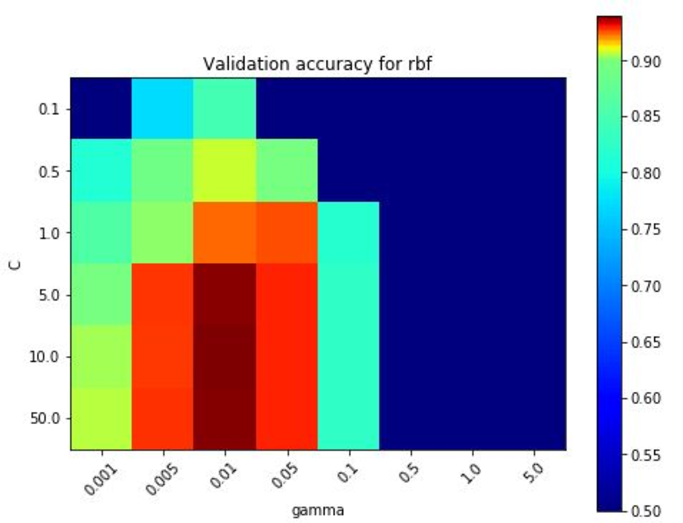
\includegraphics[width=0.8\textwidth]{figures/hm1.pdf}
\end{minipage}
\hfill
\begin{minipage}{0.49\textwidth}
  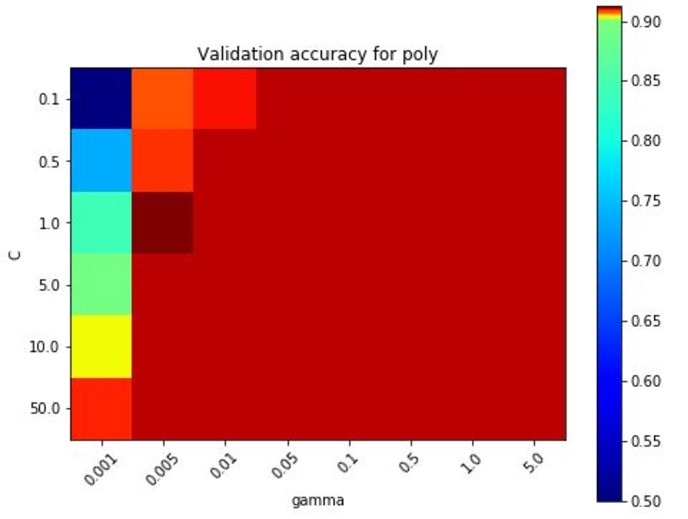
\includegraphics[width=0.8\textwidth]{figures/hm2.pdf}
\end{minipage}

Using this, we were able to obtain a $97.9\%$ accuracy.

\subsection*{MLP and CNN}

The MLP and CNN tasks where both achieved by using the
pytorch\footnote{\url{https://pytorch.org/}} library. We also performed a
gridsearch like approach to find the best parameters for each of them.

For the MLP, we finally got a model with $512$ hidden neuron and a learning rate
of $0.001$, other learning rate where not stable at all for this task.

We also go a learning rate of $0.001$ for the CNN model since higher one (like
$0.002$ or $0.007$) showed rollercoaster like curve :

\vspace*{0.2cm}

\begin{minipage}{0.49\textwidth}
  \begin{center}
    \fbox{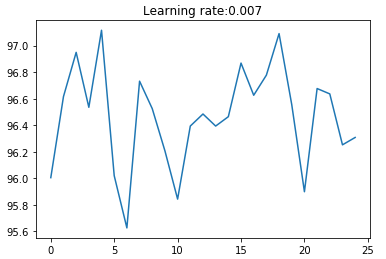
\includegraphics[width=0.6\textwidth]{figures/cnn-curve.png}}
  \end{center}
\end{minipage}
\begin{minipage}{0.49\textwidth}
Finally, we achieved a accuracy of $97.0\%$ for the MLP and $97.8\%$ for the CNN.
\end{minipage}

\subsection*{Keyword spotting}

The features we are using for this task are the suggested one : lower contour, upper
contour, black/white transitions, fraction of black pixels in the window,
fraction of black pixels between the upper and lower contour and the gradient.

The evaluation part was kind of hard to understand and to set up, since we
didn't get immediatly how to measure the quality of our solution.

We implemented our own DTW function but it was really slow and that's messed our
work too, since we had to wait between evaluation and run in order to work on
the task. The implementation is shown on the right.
\begin{pythoncode}
def __dtw(self, x, y, dist):
  len_x, len_y = len(x), len(y)
  window = [(i, j) for i in range(len_x) for j in range(len_y)]
  window = ((i + 1, j + 1) for i, j in window)
  D = defaultdict(lambda: (float('inf'),))
  D[0, 0] = (0, 0, 0)
  for i, j in window:
    dt = dist(x[i - 1], y[j - 1])
    D[i, j] = min((D[i - 1, j][0] + dt, i - 1, j),(D[i, j - 1][0] + dt, i, j -1),
    (D[i - 1, j - 1][0] + dt, i - 1, j - 1),key = lambda a: a[0])

  path = []
  i, j = len_x, len_y
  while not (i == j == 0):
    path.append((i - 1, j - 1))
    i, j = D[i, j][1], D[i, j][2]
  path.reverse()
  return D[len_x, len_y][0], path
\end{pythoncode}

\subsection*{Signature Verification}

We use the same DTW function to solve this task as the previous one, so it was
slow as well.

For the features, we computed the velocity for $x$ and $y$ as well as the
pressure, and normalize them with respect to the user.

\section*{General thoughts and feedback}

The two differents kind of exercices : implementing the algorithms by ourselves and using
existing solutions is a good approach of the project. Whit that, we can
understand the algorithms and discover various libraries to solve specific tasks
(for example, the gridsearch part or when ploting heatmaps).

As a personal feedback (Sylvain Julmy), it was hard to use the Python
programming language with the other members of the group, since I almost never
used it. Therefore reading, understanding and using the implementation of my
comrades lost me a lot of time during the tasks.

\end{document}